\documentclass[11pt,answers,addpoints]{exam}
\usepackage{color}
\usepackage{graphicx}
\usepackage[latin1]{inputenc}
\usepackage{tikz}
\usetikzlibrary{trees}
\usepackage{verbatim}
\usepackage{amsmath}

\setlength{\oddsidemargin}{-0.5in}
\setlength{\evensidemargin}{.0in} \setlength{\topmargin}{-0.5in}
\setlength{\textheight}{10in} \setlength{\textwidth}{7.5in}



\begin{document}
% Set the overall layout of the tree
\tikzstyle{level 1}=[level distance=3.5cm, sibling distance=2.5cm]
\tikzstyle{level 2}=[level distance=3.5cm, sibling distance=1.5cm]

% Define styles for bags and leafs
\tikzstyle{bag} = [text width=4em, text centered] \tikzstyle{end} =
[circle, minimum width=3pt,fill, inner sep=0pt]

\CorrectChoiceEmphasis{\color{red}\bfseries}
\bracketedpoints
\pointpoints{pt}{pts}
\setlength\answerskip{0.05ex}


\begin{flushleft}
Name:\underline{~~~~~~~~~~~~~~~~~~} \hfill PID:\underline{~~~~~~~~~~~~~~~~}\\ \vskip 1cm
Pledge: I have neither given nor received aid in this examination.\\ \vskip 1cm
Signature:\underline{~~~~~~~~~~~~~~~~~~}
\end{flushleft}

\begin{center}
{\Large {\bf CMSE381  QUIZ 2} }\\
\vspace{2ex} Oct 15th, 2021
\end{center}

\noindent {\bf Instructions:}\\
This is a closed book and closed notes examination. The best way to earn partial credits is to show all of your work. The instructor reserves
the right to remove points if not all steps are shown. The total points are 20.You have 30 minus for this QUIZ. Good luck!

\mbox{}

\makebox[5.5in]{\hrulefill}\\

\begin{questions}


\question \begin{itemize}
    \item[a] (5 pts) For a classification problem with $K = 2$ ($Y \in \{0, 1\}$) and loss function of $\sum_{i = 1}^n I(y_i \neq C(x_i))$, what is the oracle (the best classifier)?
    \item[b] (10 pts) For a classification problem with $K = 2$, if we know Type I erorr will cost \$10 while Type II error will cost \$20. Derive the new oracle classifier which minimizes this cost. (Please write your answer on a white paper)
    \item[c] (5 pts) If $K = 3 \ \ (Y \in \{0, 1, 2 \}$), will you prefer Logistic regression or LDA? Justify your answer
\end{itemize}
\vspace{3in}

\newpage
\question[10] We want to build a binary classification model for the following data. Should we use a LDA or QDA model? Justify your choice.(Please write your answer on a white paper)

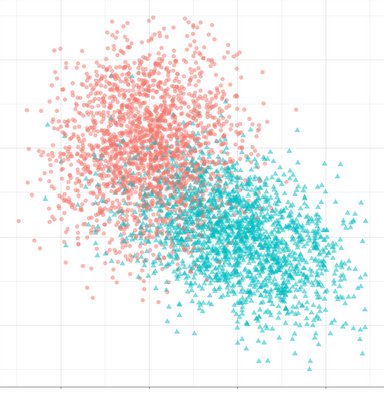
\includegraphics[scale=2]{fig1.png}
\vspace{2in}
\question[5] We are trying to predict whether a patient will have a heart attach within one year. We have tried four different methods on a training dataset and have the following ROC curves. Which curve has the best performance on this training set? Justify your answer.\\
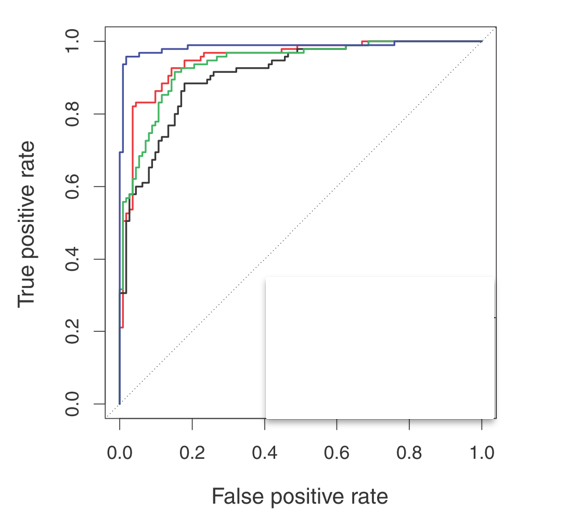
\includegraphics[width=5cm]{./Picture3.png}

\newpage
	
	


\question[10] We want to study the relationship between cups of coffee ($Y$) a people may drink per day and the stress score ($X$). Here $X$ and $Y$ are
random quantities. From Dr. Sparty's research, we think the relationship is $$Y = \alpha \exp(\beta \sin^2 (X) + 100).$$ We then collected 10000 data $\{(x_1, y_1), \ldots (x_{10000}, y_{10000}) \}$ and can estimate $\hat{\alpha}$ and $\hat{\beta}$ from this data. If we want to quantify the accuracy of our estimate of $\alpha$ and $\beta$ in terms of confidence interval, what procedure will you follow to obtain it (Validation set, Cross validation, bootstrap, forward selection, backward selection, best subset, etc)? Outline your procedure. (Please write your answer on a white paper)
\vspace{2in}

\question[5] If we want to estimate the variance of testing error for our model, should we use CV or Bootstrap? Which method will produce a larger estimate of the testing error? Justify your answer

\vspace{1 in}

\question (Extra 2 pts) Prove that when sample size $n$ goes to infinity,  a bootstrap dataset will contain $1 - e^{-1}$  of original data. 

\end{questions}



\end{document}
